% ------------- comparaison_p_correl_s_aleatoire_aucune ----------
\begin{figure}[htb!] 
\centering
% aleatoire aucune = aleatoire unitaire
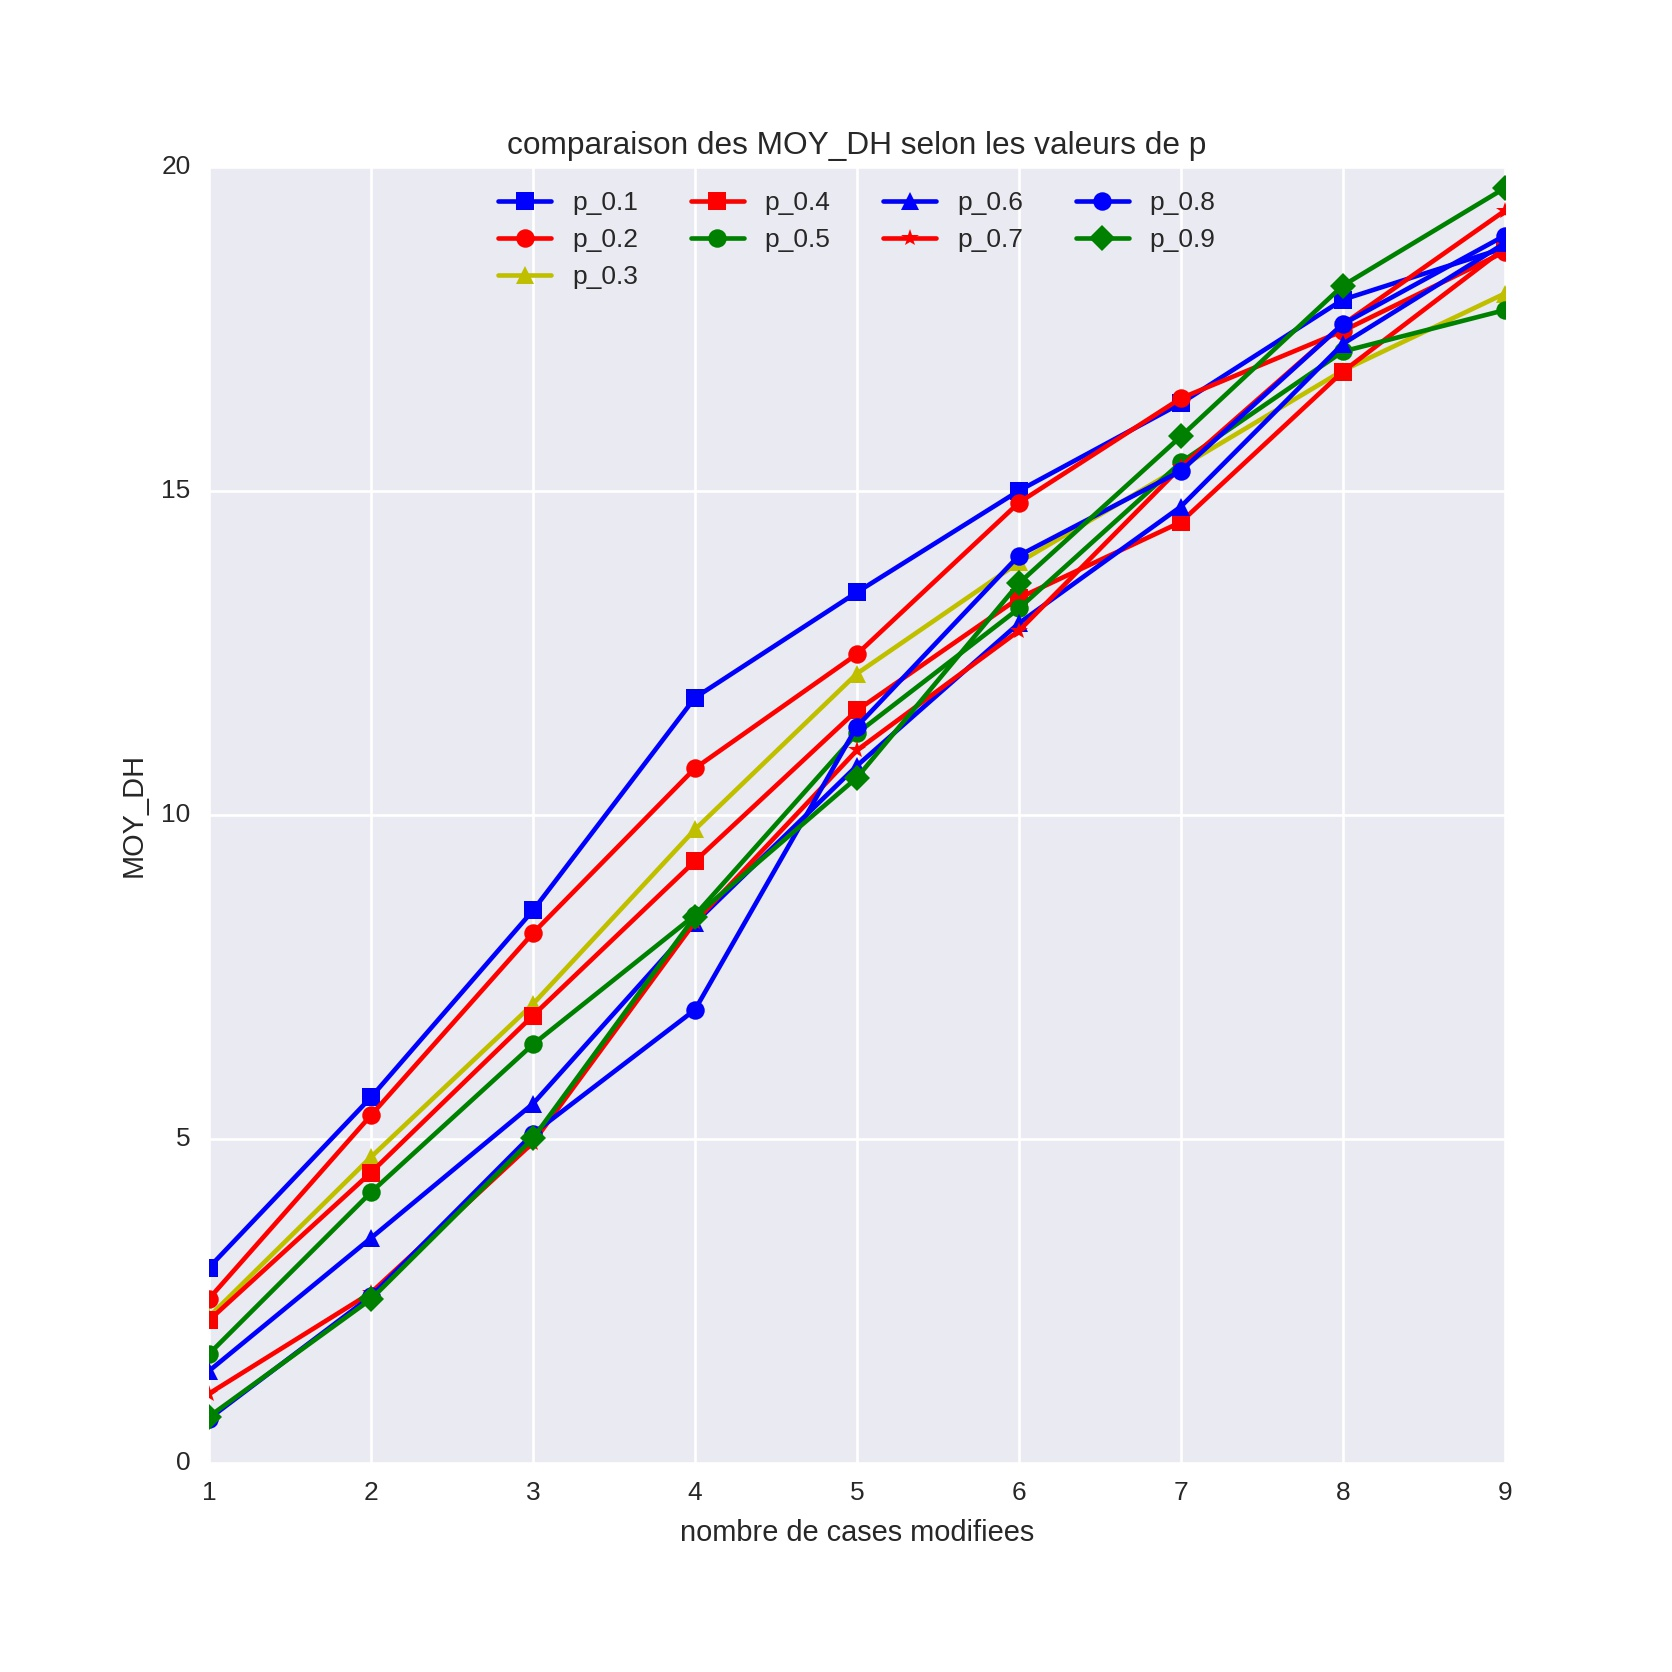
\includegraphics[scale=0.25]{comparaison_p_correl_s_aleatoire_aucune.jpeg}
\caption{ Comparaison des diff\'erentes repartitions des $k \in \{1,\cdots,9\}$ cases fausses positives et fausses n\'egatives avec l'approche {\em al\'eatoire sans remise} et la fonction de co\^ut {\em unitaire}. }
\label{comparaison_p_correl_s_aleatoire_aucune} 
\end{figure}
%\FloatBarrier
% ------------- comparaison_p_correl_s_aleatoire_aucune ----------


Nous mesurons l'influence des fonctions de co\^ut sur nos distances de Hamming.
Pour ce faire, nous appliquons les fonctions de co\^ut {\em unitaire}, {\em ajout} et {\em suppression} (voir tableau \ref{tab:recapApprocheCorrection}) pour en d\'eduire les valeurs de $p$ qui sont favorables \`a l'algorithme de correction c'est-\`a-dire qui minimisent les distances de Hamming.
\newline

Nous consid\'erons d'abord la fonction {\em unitaire}.
La figure \ref{comparaison_p_correl_s_aleatoire_aucune} repr\'esente l'\'evolution des distances de Hamming selon les diff\'erentes valeurs de $p$.  Les courbes de $p$ sont \'eloign\'ees pour $k \le 5$ et au d\'el\`a de  $k > 5$, les courbes se rapprochent. 
En effet, 
pour $k \le 5$, $43.4\%$ des cases {\em fausses n\'egatives} en moyenne sont corrig\'ees pour $p\in \{0.7, 0.9\}$ et pour $p=0.8$, cette moyenne est de $45.5\%$. Quant aux cases {\em fausses positives}, seulement $10\%$ des cases sont corrig\'ees. 
Ces moyennes sont plus \'elev\'ees que celles obtenues avec $p<0.7$.  
En effet, seulement $19.32\%$ des cases {\em fausses positives} et $38\%$ des cases  {\em fausses n\'egatives} sont corrig\'ees avec  $p<0.7$. 
 L'algorithme de correction ajoute beaucoup d'ar\^etes pour $p \ge 0.7$ par rapport \`a $p<0.7$ parce que le nombre de cases {\em fausses n\'egatives} dans la matrice du graphe de corr\'elation est \'elev\'e pour $p<0.7$ sachant que le co\^ut d'ajout  d'une ar\^etes est de $1$.
\newline
De m\^eme, pour $k > 0.5$, $80\%$ des cases erron\'ees sont des cases {\em fausses n\'egatives} apr\`es l'algorithme de correction.  L'algorithme privil\'egie l'ajout  \`a la suppression d'ar\^etes. 
\newline
La fonction {\em unitaire} a peu d'influence sur les variations des distances de Hamming quelque soit les valeurs de $p$.  

% ------------- comparaison_p_correl_s_aleatoire_ajout -----------
\begin{figure}[htb!] 
\centering
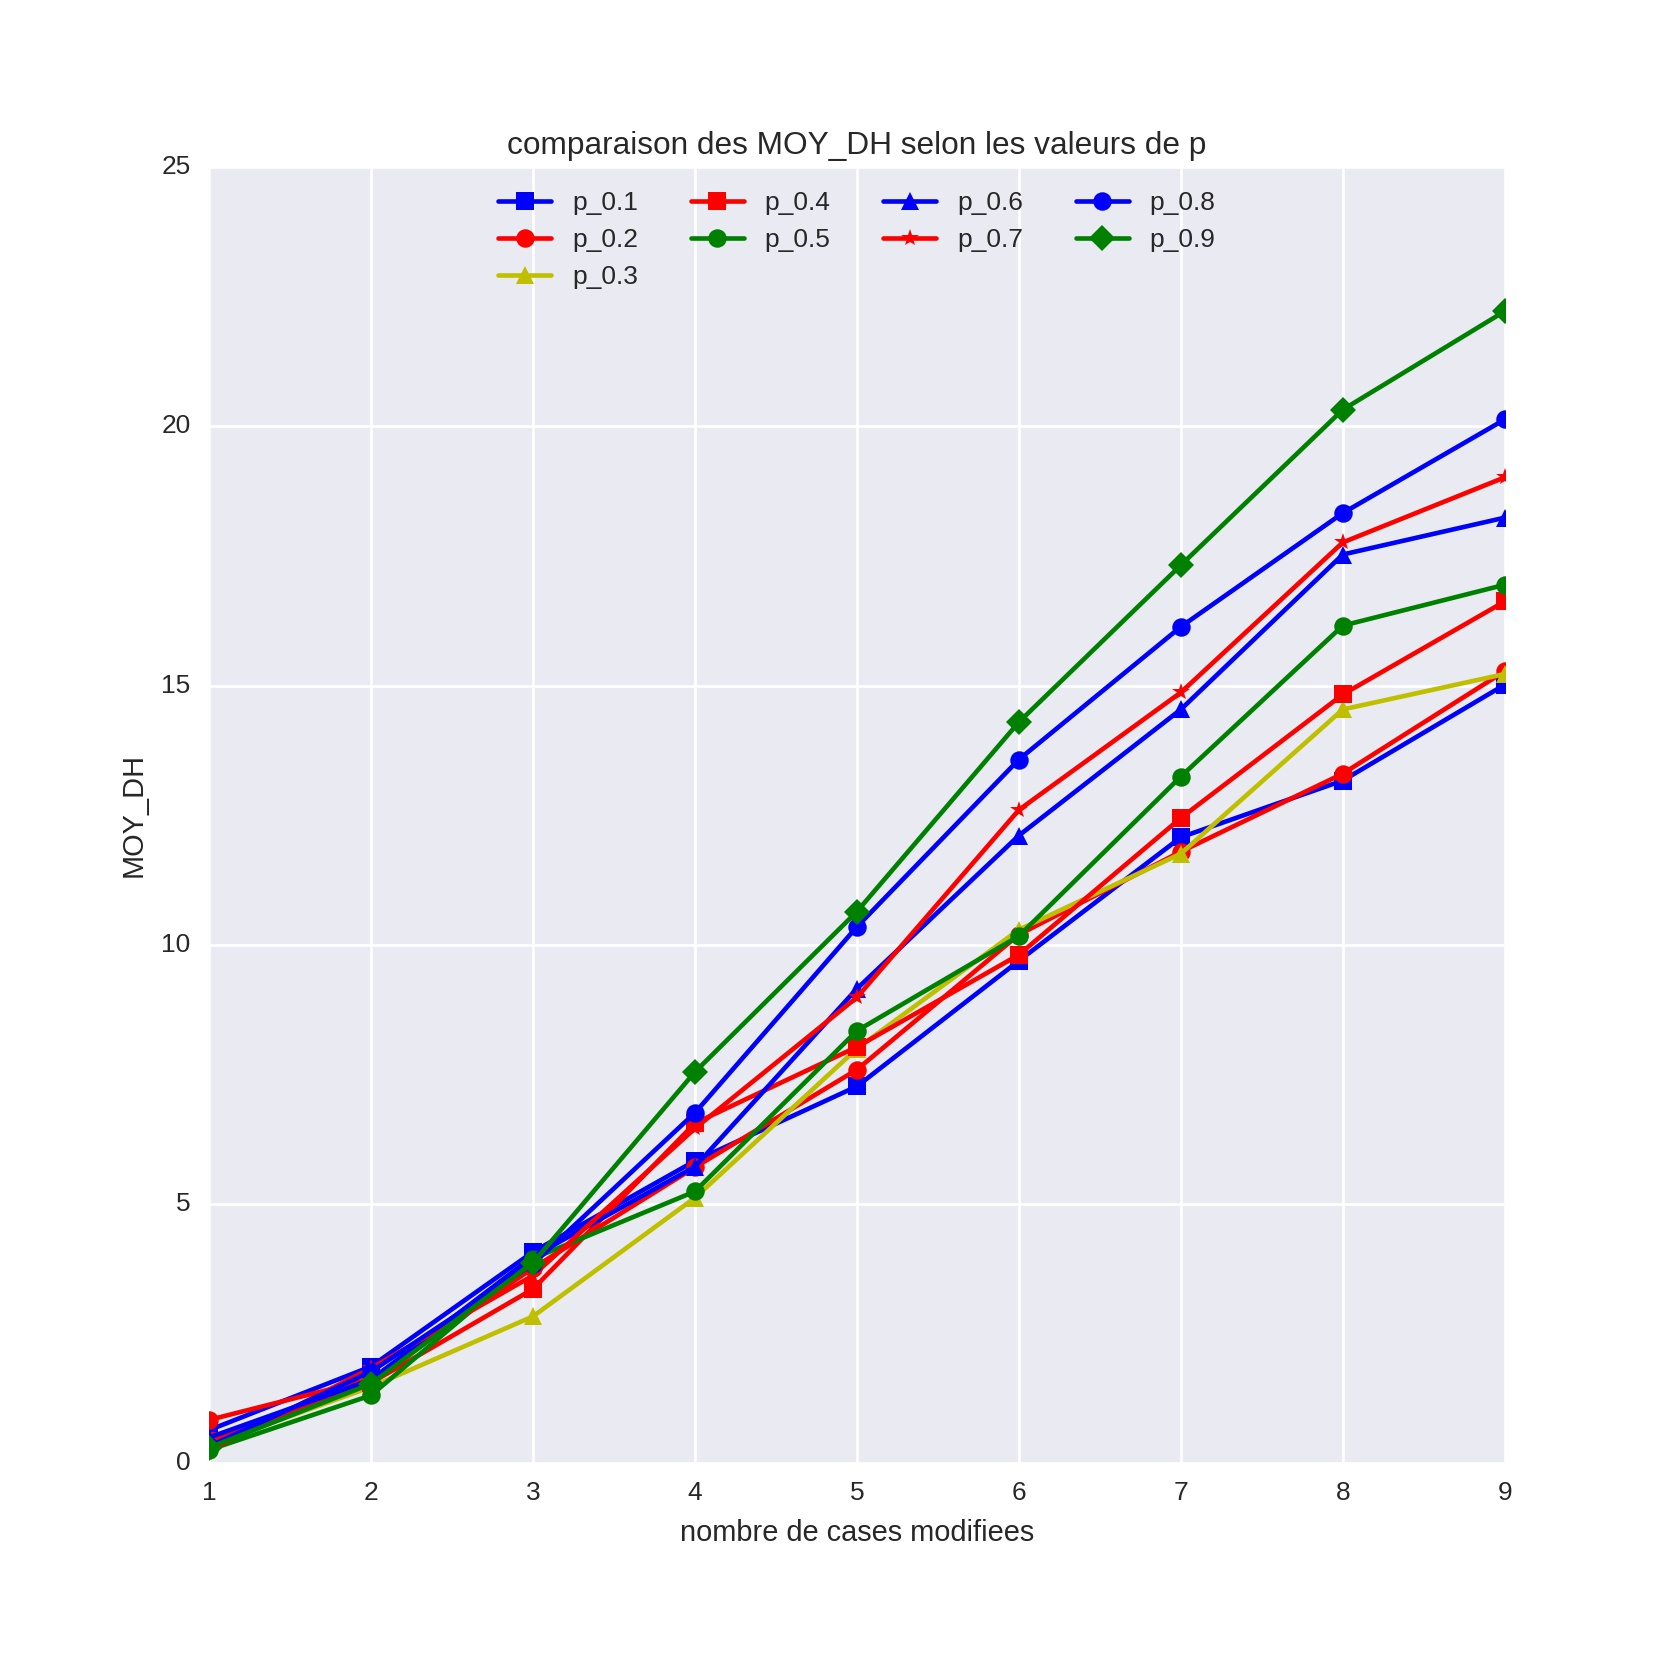
\includegraphics[scale=0.25]{comparaison_p_correl_s_aleatoire_ajout.jpeg}
\caption{ Comparaison des diff\'erentes repartitions des $k \in \{1,\cdots,9\}$ cases fausses positives et fausses n\'egatives avec l'approche {\em al\'eatoire sans remise} et la fonction de co\^ut {\em ajout}.  }
\label{comparaison_p_correl_s_aleatoire_ajout} 
\end{figure}
%\FloatBarrier
% ------------- comparaison_p_correl_s_aleatoire_ajout -----------

La figure \ref{comparaison_p_correl_s_aleatoire_supp} correspond \`a la fonction {\em suppression} et elle a le m\^eme comportement que la fonction {\em unitaire} parce que toutes les courbes divergent quand $k \le 5$ et convergent quand  $k > 5$. Ici nous remarquons aussi que nous avons en moyenne beaucoup de cases {\em fausses n\'egatives} \`a la fin de l'algorithme de correction. 
Avec la fonction {\em suppression}, nous constatons que le nombre moyen de cases {\em fausses n\'egatives} \`a la fin de l'algorithme de correction est largement sup\'erieur au nombre de cases {\em fausses n\'egatives} modifi\'ees dans la matrice $M_{k,p,\alpha}$.
Cependant, le nombre de ces cases {\em fausses n\'egatives}  ($39.4\%$ en moyenne) \`a la fin de l'algorithme de correction est inf\'erieur au nombre de cases corrig\'es {\em fausses n\'egatives}  ($47.7\%$ en moyenne) avec la fonction {\em unitaire}. 
Cette baisse provient majoritairement de la position des sommets \`a corriger dans ${\cal C}$. 
En effet, il existe des chaines simples de longueur $2$ entre certains sommets de  ${\cal C}$.  Une ar\^ete de chacune des chaines est supprim\'ee afin que la compression de deux cliques fournisse une nouvelle clique de ${\cal CC}$. Cela fait que les ar\^etes incidentes ont leurs sommets de ${\cal CC}$ et ces ar\^etes sont supprim\'ees une fois sur deux au minimum. 
La fonction {\em suppression} donne le m\^eme r\'esultat que la fonction {\em unitaire}.
%\newline

% ------------- comparaison_p_correl_s_aleatoire_supp  ----------
\begin{figure}[htb!] 
\centering
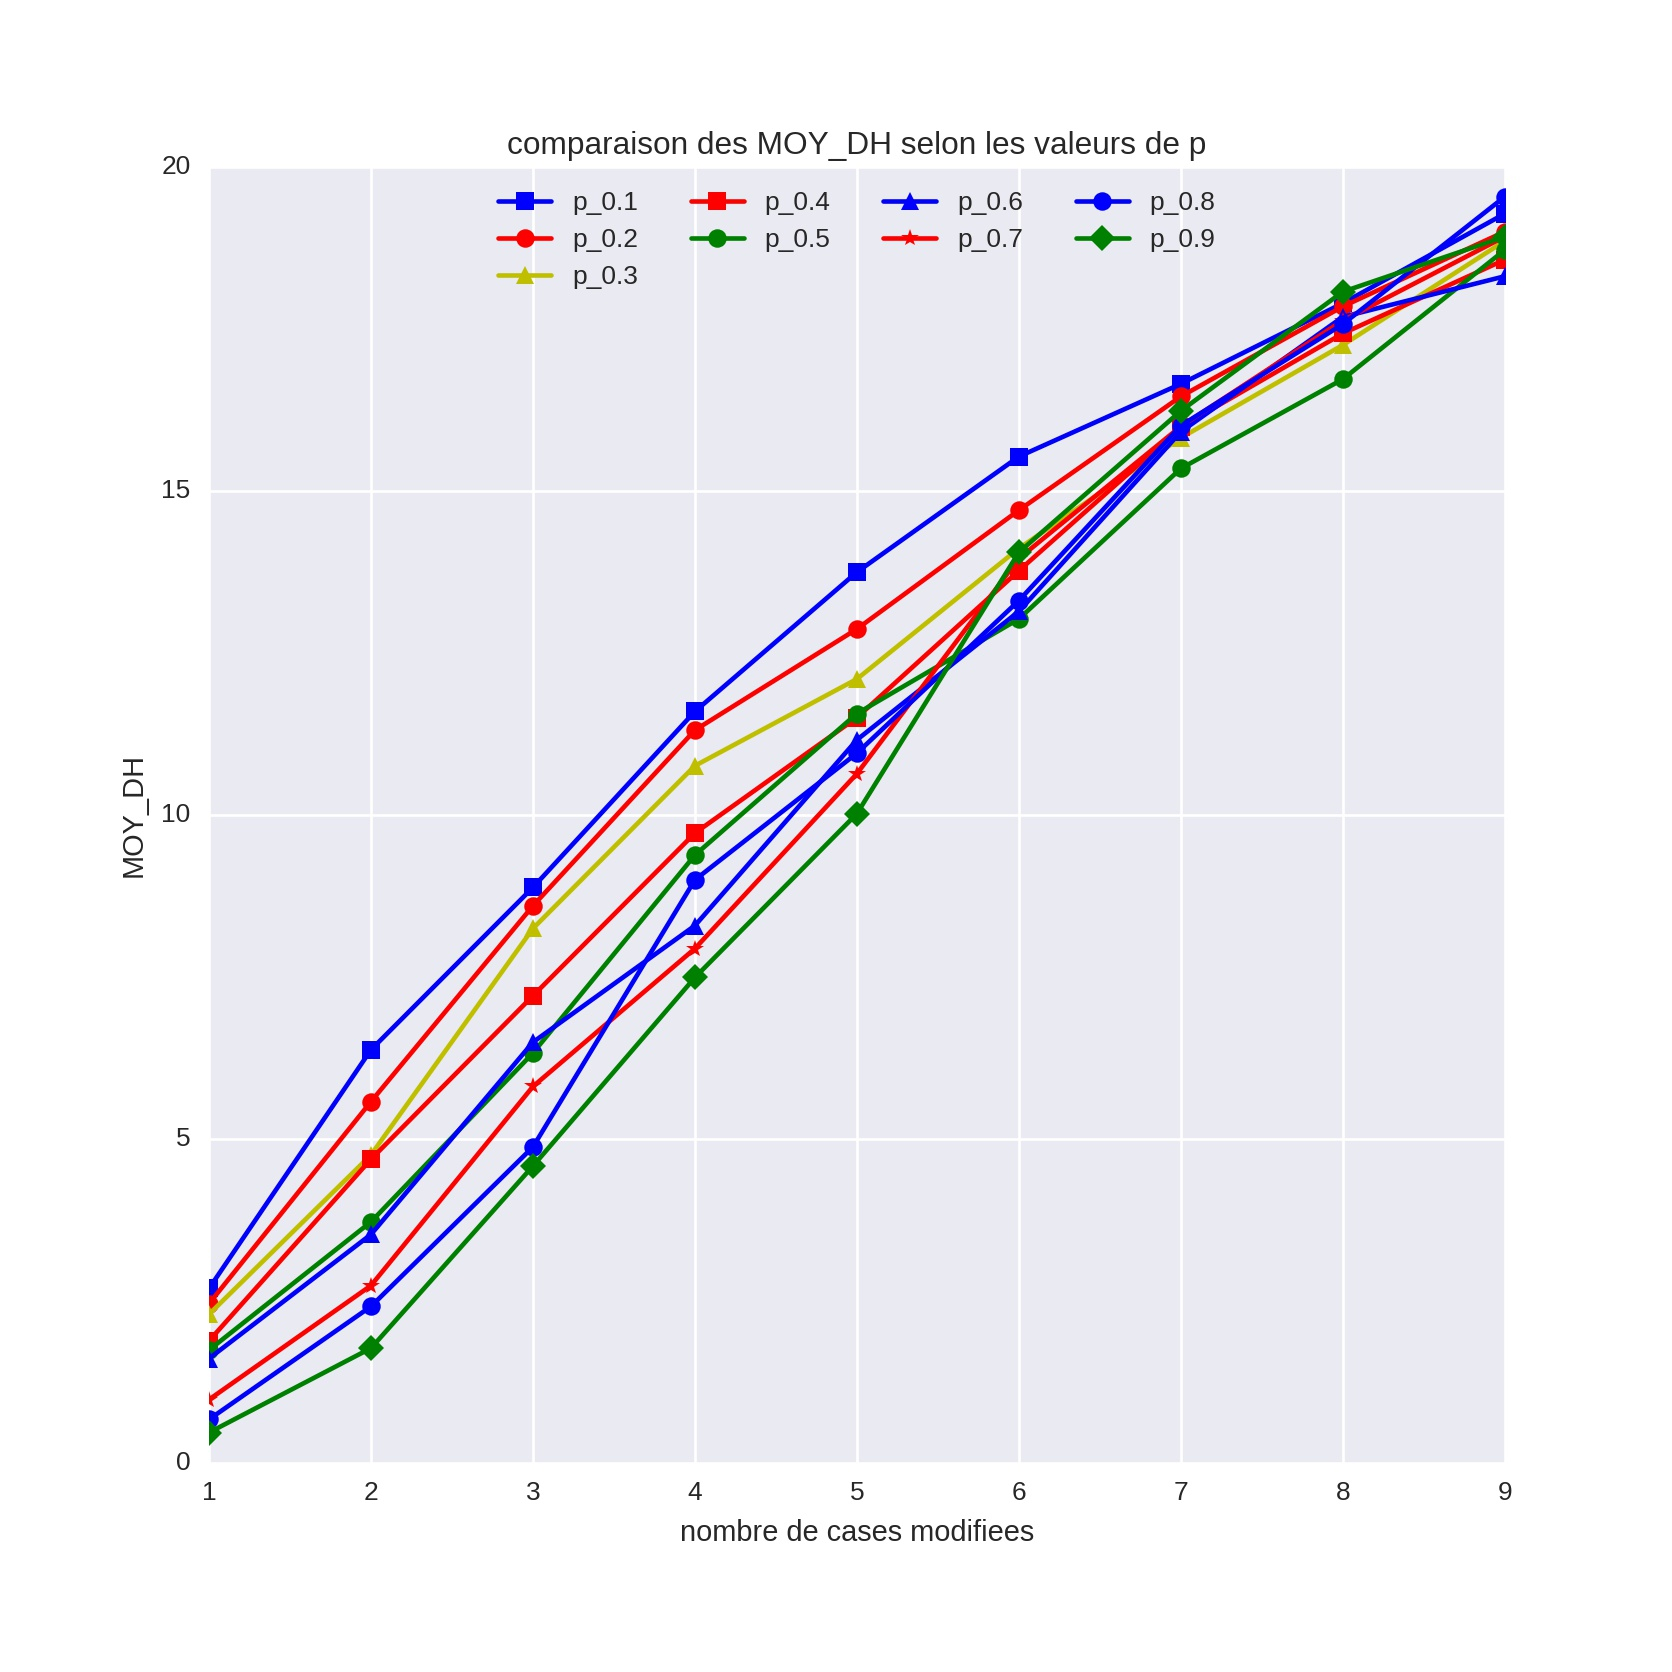
\includegraphics[scale=0.25]{comparaison_p_correl_s_aleatoire_supp.jpeg}
\caption{ Comparaison des diff\'erentes repartitions des $k \in \{1,\cdots,9\}$ cases fausses positives et fausses n\'egatives avec l'approche {\em al\'eatoire sans remise} et la fonction de co\^ut {\em suppression}. }
\label{comparaison_p_correl_s_aleatoire_supp} 
\end{figure}
%\FloatBarrier
% ------------- comparaison_p_correl_s_aleatoire_supp  ----------

Dans la figure \ref{comparaison_p_correl_s_aleatoire_ajout} associ\'ee \`a la fonction {\em ajout}, les courbes divergent quand $k$ est croissant.
En effet, des ar\^etes {\em fausses n\'egatives}  sont ajout\'ees \`a $G_{k,p,\alpha}$ pour $p \ge 0.4$ pendant la correction. Alors les distances $moy\_DH_{k,p}$ augmentent car le nombre de cases  {\em fausses n\'egatives} augmente et aussi plus de  $40\%$ des cases {\em fausses positives} ne sont pas supprim\'ees.  
Par ailleurs, les courbes convergent vers $0$ quand $k \le 4$. La baisse des valeurs moyennes des distances de Hamming est le r\'esultat de la correction des cases modifi\'ees dans $M_{k,p}$. N\'eanmoins, l'algorithme corrige majoritairement des cases {\em fausses n\'egatives} lorsque toutes les cases modifi\'ees ne parviennent pas \`a \^etre corrig\'ees. 
\newline

{\bf Conclusion} : nous ne pouvons pas conclure que les valeurs de $p$ ont une influence sur la correction des $k$ cases modifi\'ees car les fonctions de co\^ut {\em unitaire} et {\em suppression} font converger l'une vers l'autre leurs distances de Hamming avec l'augmentation du nombre de cases modifi\'ees. Toutefois, la fonction de co\^ut {\em ajout} fait diverger nos courbes sans cr\'eer un \'ecart significatif de distances entre ses courbes. 



%
%Consid\'erons $p \in [0,1]$, la variable de repartition des $k$ cases modifi\'ees. 
%$p = 0.1$ signifie que $10\%$ des $k$  cases modifi\'ees ajoutent des ar\^etes au graphe  $G_{k,p, \alpha}$ (cases {\em fausses positives}) et les $90\%$ des cases restantes suppriment des ar\^etes du graphe (cases {\em fausses n\'egatives}). Nous pr\'ecisons \'egalement que la fonction de co\^ut est {\em unitaire}.
%La figure \ref{comparaison_p_correl_s_aleatoire_aucune} r\'esume 
%l'\'evolution des distances de Hamming $moy\_DH$ en fonction des $k \in \{1,\cdots,9\}$ cases modifi\'ees pour diff\'erentes valeurs de $p$. 
%Les courbes sont croissantes et  la courbe de $p = 0.8$ donne les distances de Hamming minimales  \`a partir de $k \le 4 $. Au d\'el\`a de $k > 4$, les courbes se rapprochent les unes des autres et il est difficile de d\'eterminer la valeur $p$ qui fournit la plus petite distance.
%En effet, pour  $k \le 4$, les courbes divergent parce que les cases modifi\'ees ne sont pas corrig\'ees et d'autres cases sont modifi\'ees. Cela augmente l'ensemble de cases ({\em fausses n\'egatives et fausses positives}).
%N\'eammoins, les cases modifi\'ees sont corrig\'ees pour $k > 4$ et cela entraine que les courbes se rapprochent.
%Le probl\`eme de la bonne repartition semble \^etre difficile \`a trouver pour la fonction de cout {\em unitaire}. Nous allons appliquer d'autres fonctions de co\^ut pour d\'eduire une valeur de $p$ acceptable qui minimise les distances de Hamming.
%\newline
%La fonction de co\^ut {\em suppression} a le m\^eme comportement que la fonction {\em unitaire} comme indiqu\'e dans la figure \ref{comparaison_p_correl_s_aleatoire_supp}. La divergence des courbes se produit pour $k \in \{1,\cdots,5\}$ et la courbe de $p = 0.9$ fournit les distances de Hamming minimales (sa courbe est en dessous des autres). \`A partir de $k > 5$, les courbes se rapprochent et la meilleure courbe est  celle de $p = 0.5$. 
%Nous l'expliquons par la modification des cases {\em fausses n\'egatives} pour $p =0.9$ et par  l'ajout d'ar\^etes pour $p = 0.5$.
%\newline
%Dans la figure \ref{comparaison_p_correl_s_aleatoire_ajout} associ\'ee \`a la fonction de co\^ut {\em ajout}, les courbes divergent quand $k$ est croissant.
%En effet, des ar\^etes suppl\'ementaires  sont ajout\'ees \`a $G_{k,p}$ pour $p \ge 0.4$. Les distances $moy\_DH$ augmentent car plus de  $40\%$ des cases {\em fausses positives} ne sont pas supprim\'ees.  
%Par ailleurs, pour $p = 0.1$, la distance de Hamming moyenne est de $1.421,2.305,3.109$ pour $k = 1,2,3$ respectivement et pour $k \ge 4$, cette distance augmente d'environ $1.5 \times k$.
%L'algorithme corrige autour de $20\%$ les cases {\em fausses n\'egatives} et les ar\^etes de la distance de Hamming correspondent majoritairement aux cases {\em fausses positives} modifi\'ees  pendant la phase de correction.
%\newline
%Nous ne pouvons pas conclure que la repartition des $k$ cases modifi\'ees de $M_{LG}$ a un impact sur la correction des sommets $noeud \in {\cal C}$ car les fonctions de co\^ut {\em unitaire} et {\em suppression} font converger nos distances de Hamming avec l'augmentation du nombre de cases modifi\'ees. Toutefois, la fonction de co\^ut {\em ajout} fait diverger nos courbes sans cr\'eer un \'ecart significatif de distances entre ses courbes.  


% ----- partir a envoyer 



%% comparaison de p_correl sur la methode de permutation aleatoire
%%% ---- pas encore REPROGRAMMER -- utiliser la fonction de cout unitaire
%\begin{figure}[htb!] 
%\centering
%% meilleur probabilite p parmi les [0.0, 0.1, 0.2, ...., 1.0]
%% a changer par des chemins relatifs
%%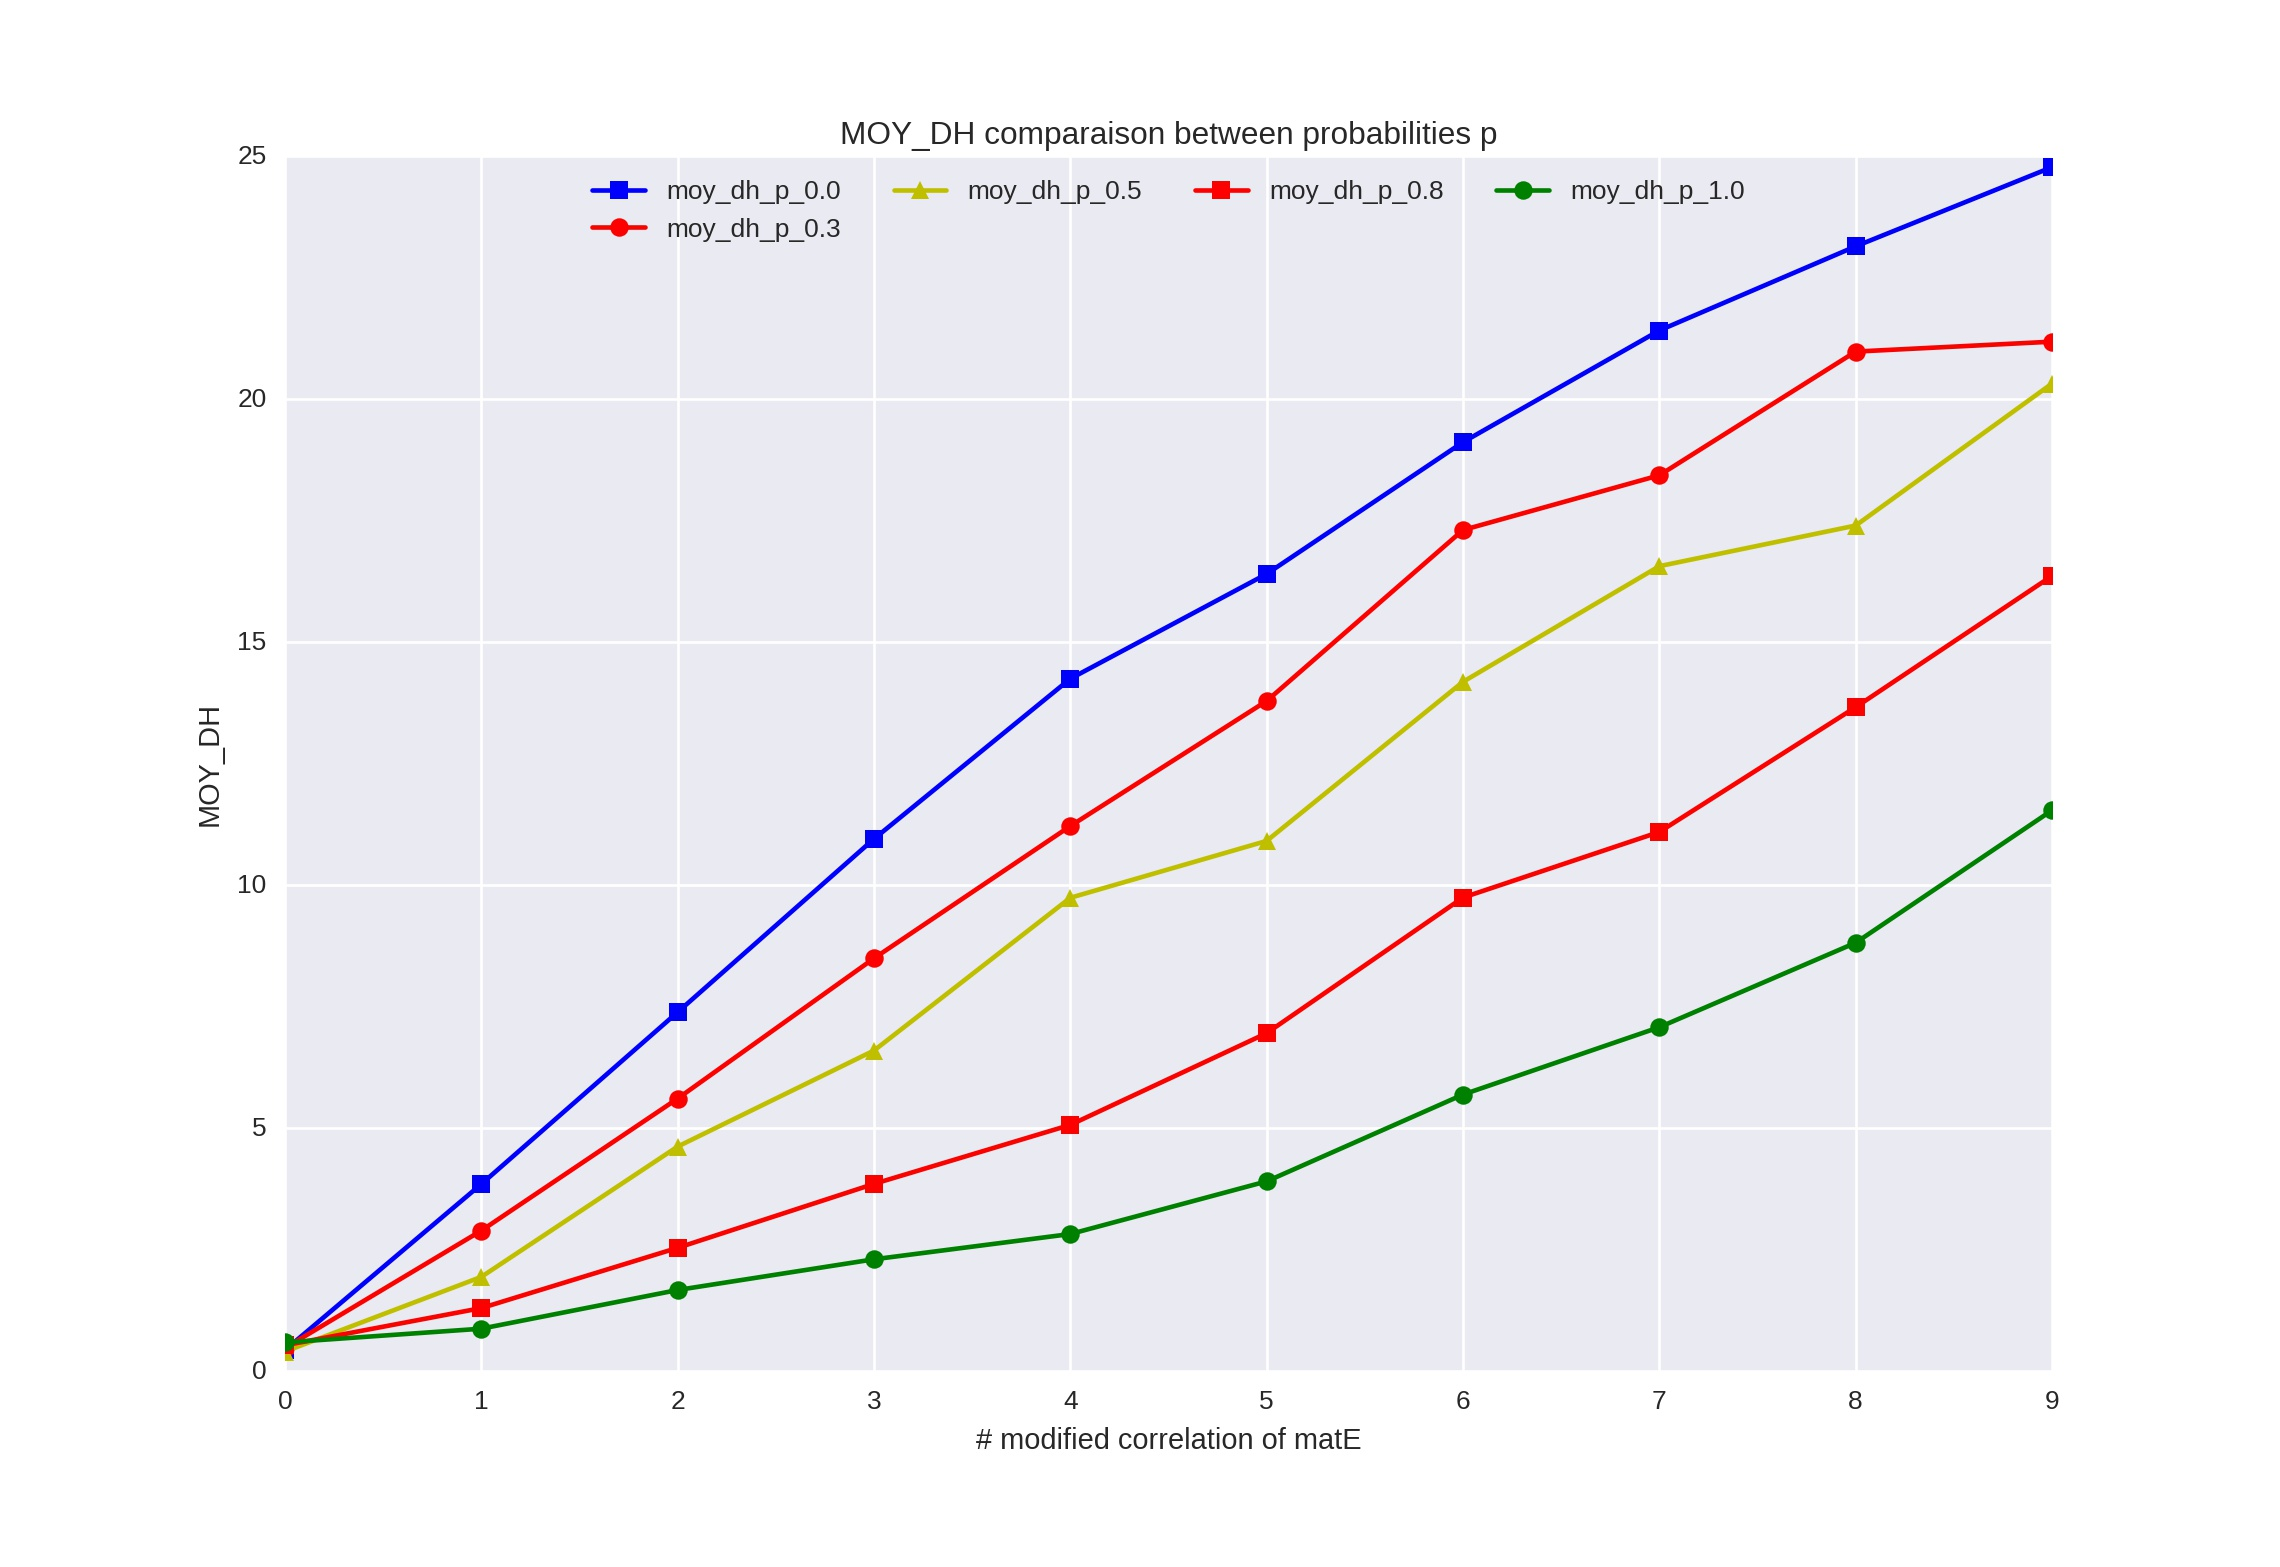
\includegraphics[scale=0.25]{permut_aleatoire_coutMin_degreMin_fct_cout_normal_500G/aleatoire/courbes/comparaison_probabilities_p_00_10_moy_dh_aleatoire_p_10.jpeg}
%%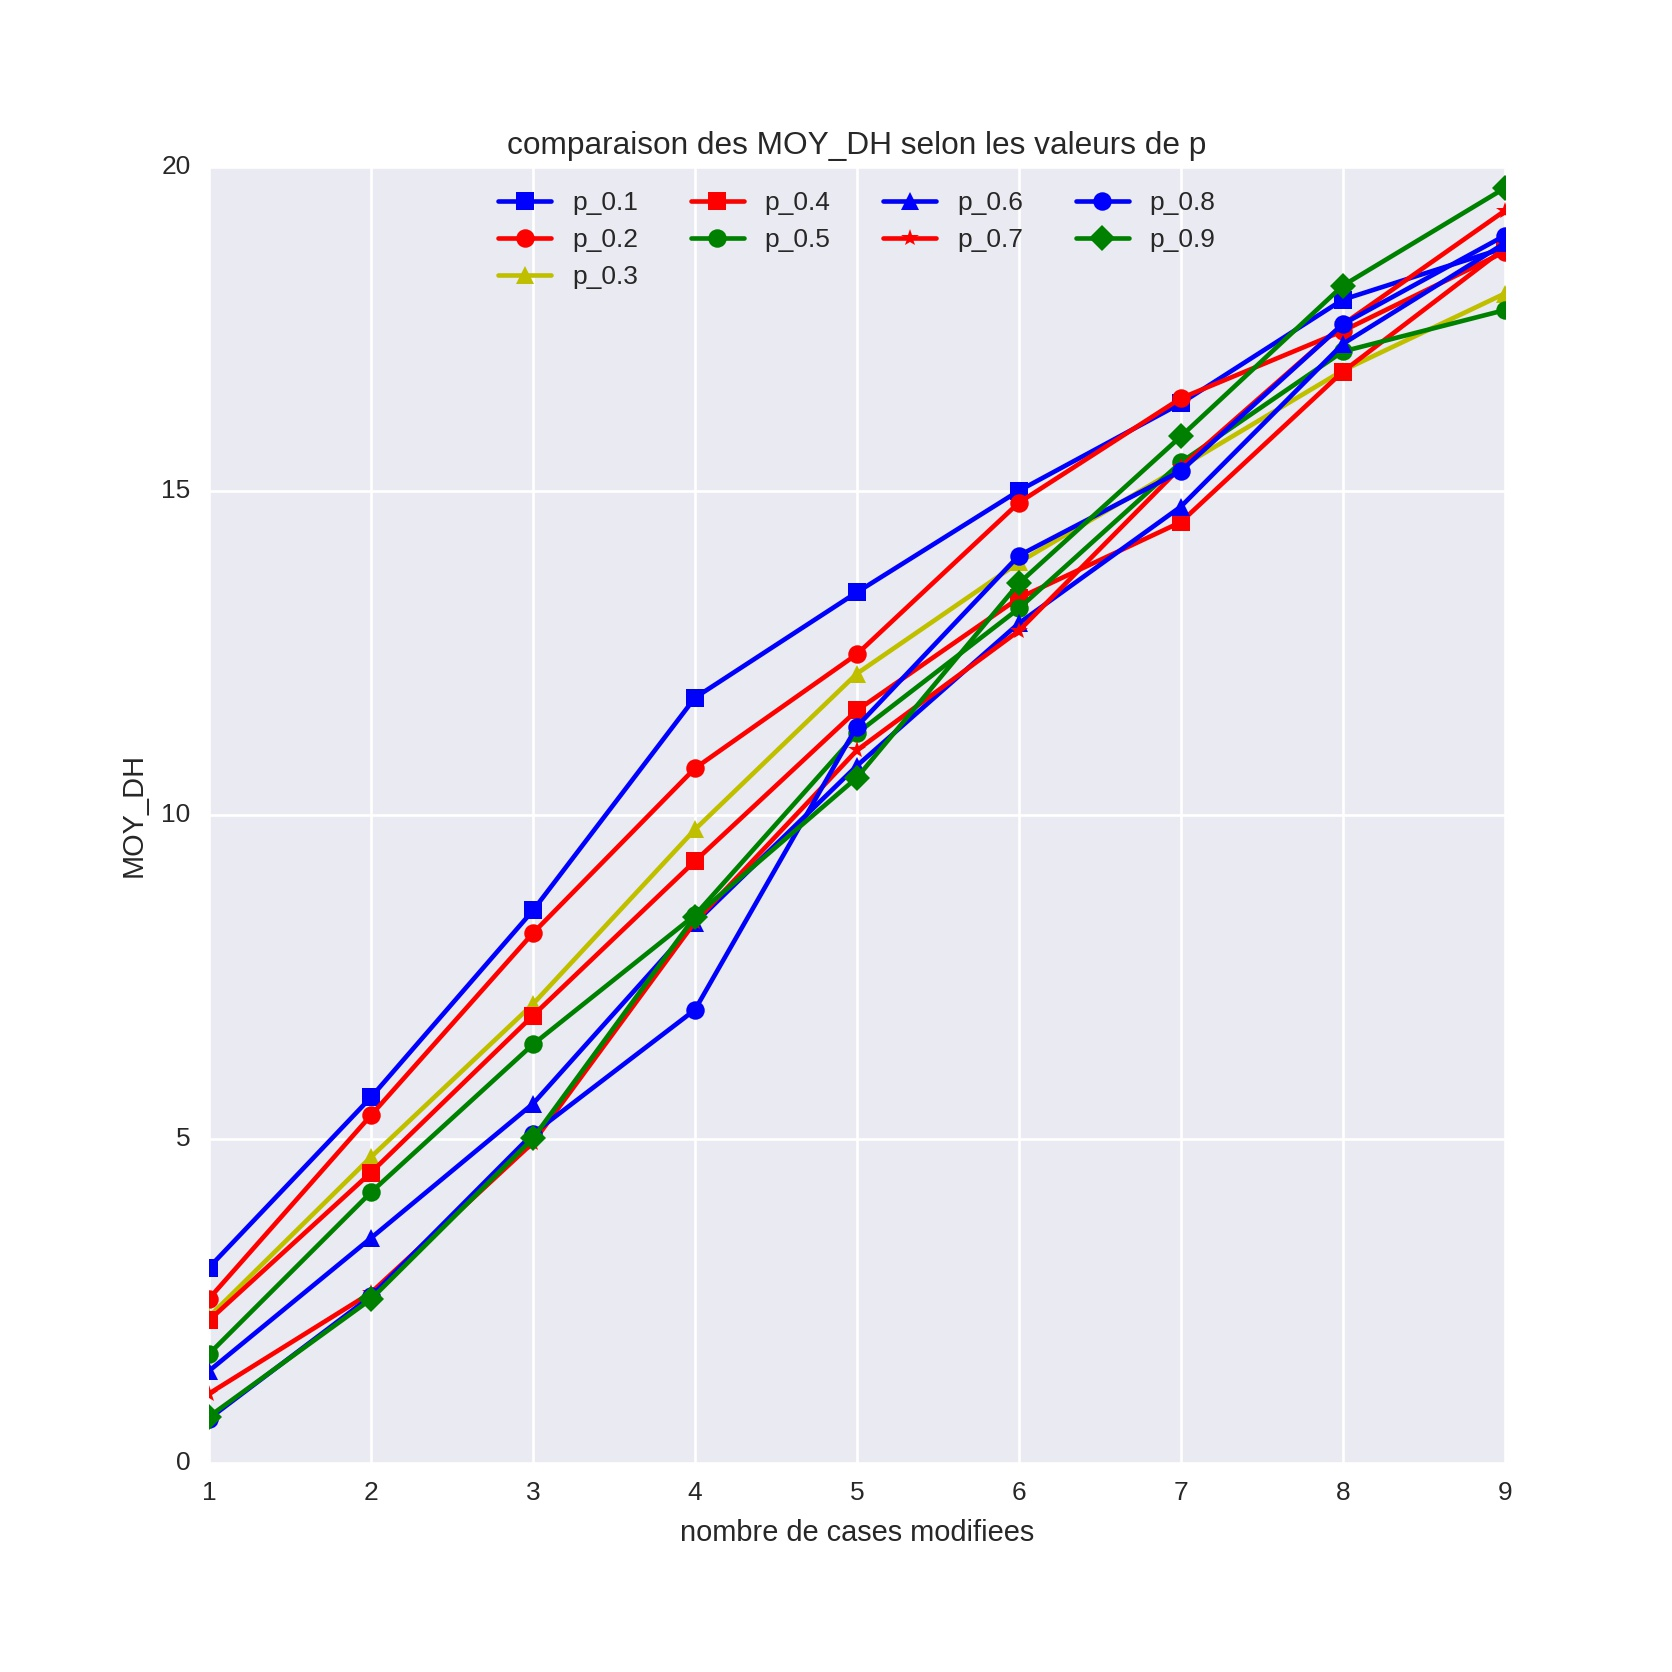
\includegraphics[scale=0.25]{comparaison_p_correl_s_aleatoire_aucune.jpeg}
%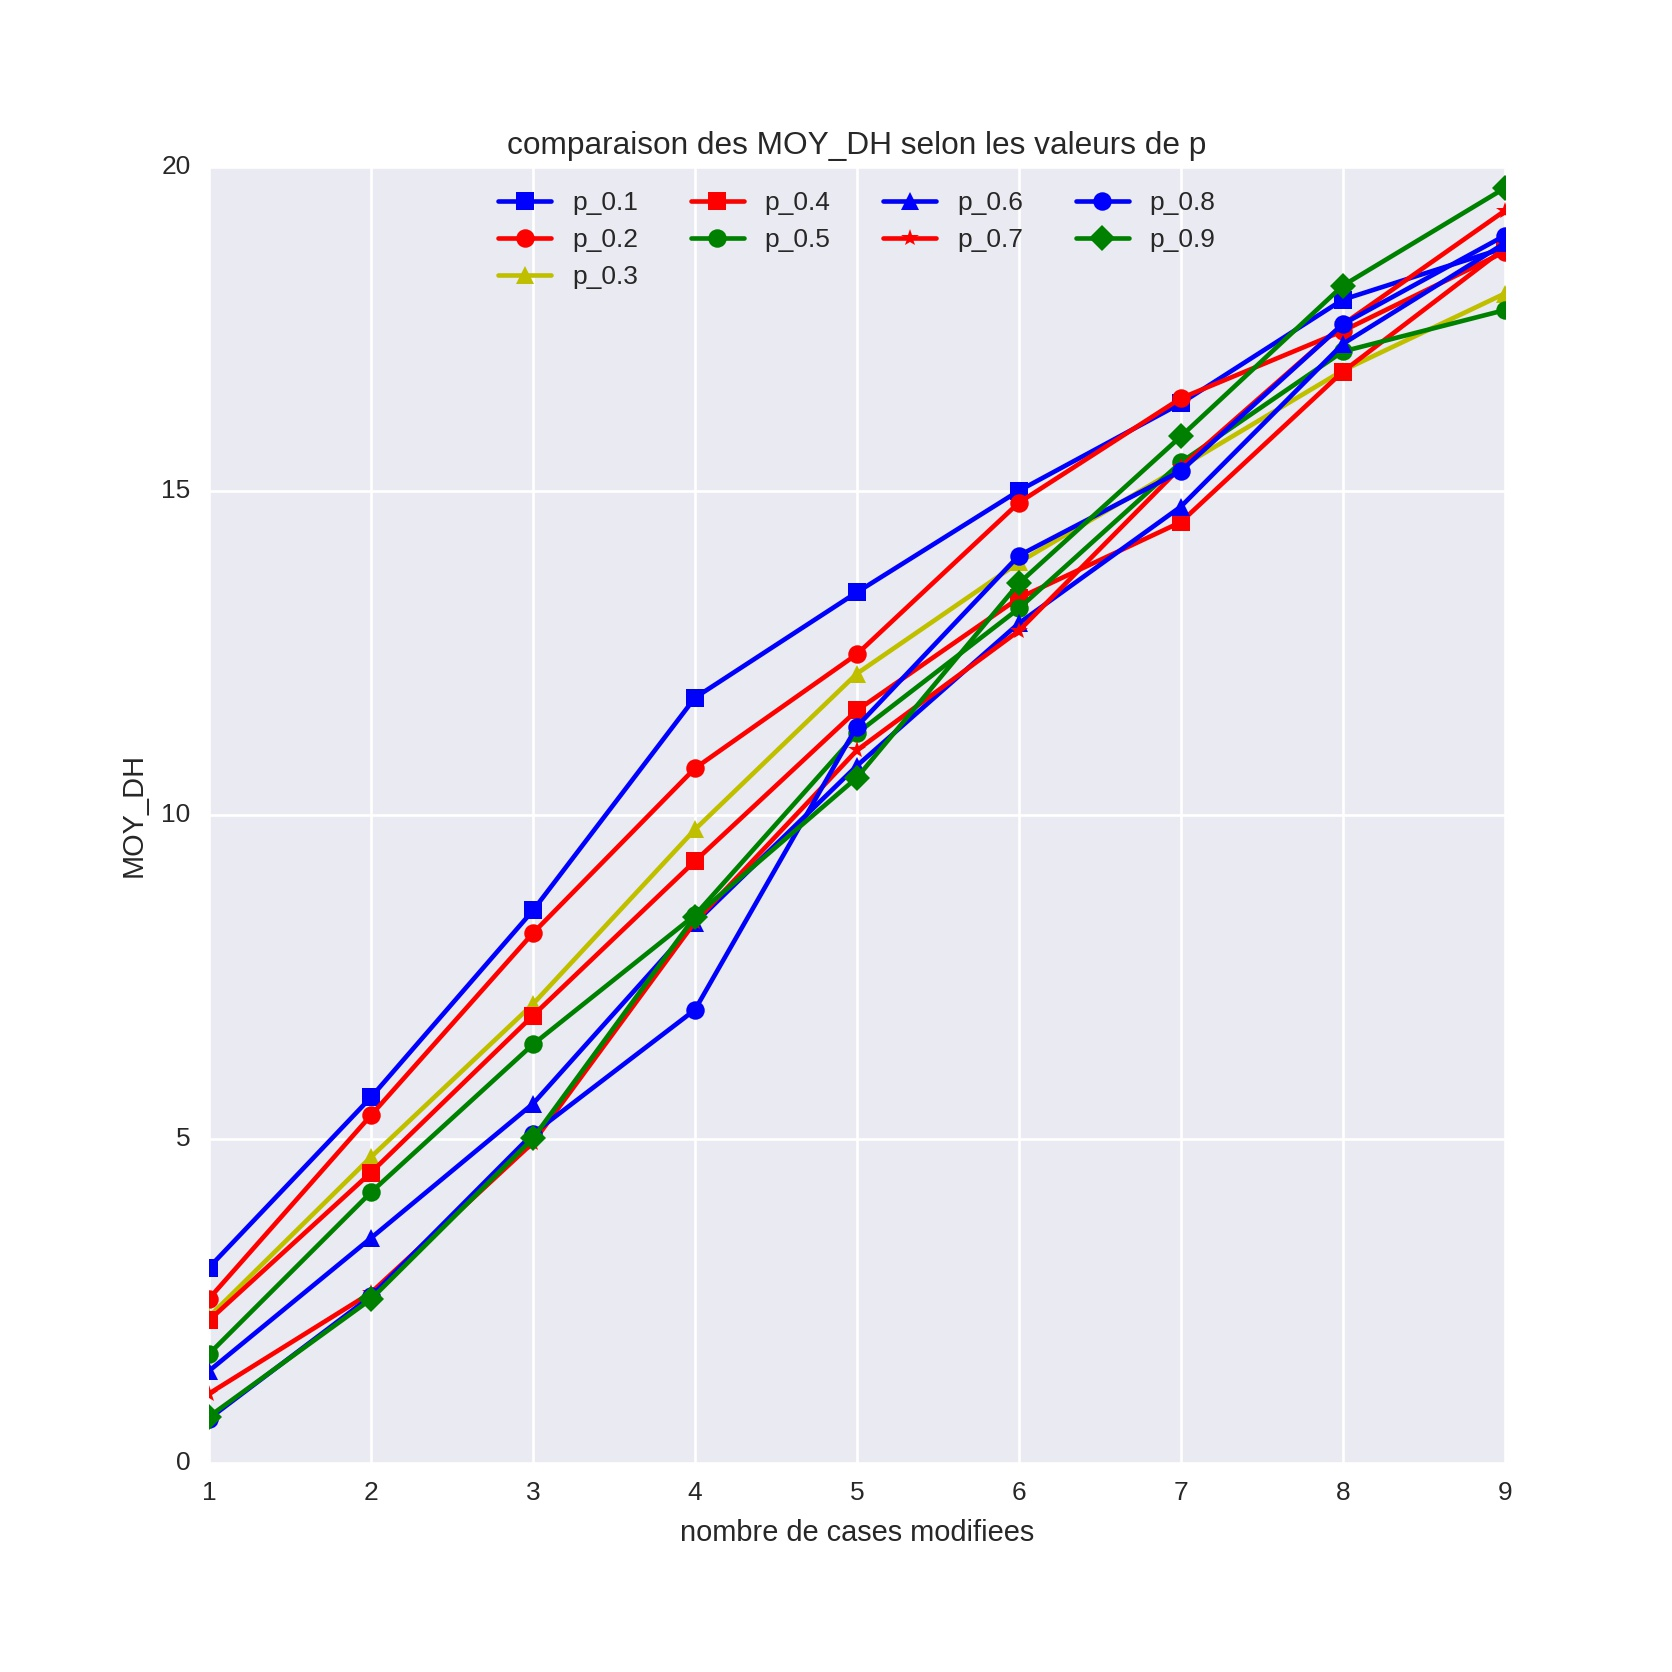
\includegraphics[scale=0.25]{comparaison_p_correl_s_aleatoire_aucune.jpeg}
%\caption{ Comparaison des diff\'erentes probabilit\'es d'ajout $k \in [1,9]$ de corr\'elations fausses positives et fausses n\'egatives sur la m\'ethode de permutation al\'eatoire }
%\label{comparaison_p_correl_s_aleatoire_aucune} 
%\end{figure}
%%% ---- pas encore REPROGRAMMER
%Consid\'erons la variable $p\_correl \in [0,1]$. 
%$p\_correl = 0.1$ signifie que $10\%$ des $k$  cases modifi\'ees ajoutent des ar\^etes au graphe  $G_{k,p\_correl, \alpha}$ (erreurs {\em fausses positives}) et les $90\%$ des cases restantes suppriment des ar\^etes du graphe (erreurs {\em fausses n\'egatives}). Nous pr\'ecisons \'egalement que  l'ajout et la suppression d'ar\^etes ont le m\^eme co\^ut de traitement c'est-\`a-dire $1$.
%La figure \ref{comparaison_p_correl_s_aleatoire_aucune} r\'esume 
%l'\'evolution des distances de Hamming $moy\_DH$ en fonction des $k \in [1,9]$ cases modifi\'ees pour diff\'erentes valeurs de $p\_correl$. 
%Les courbes sont croissantes et nous constatons que pour $k \le 4 $, la courbe de $p\_correl = 0.8$ donne les distances de Hamming minimales. Au d\'el\`a de $k > 4$, les courbes se rapprochent les unes des autres et il est difficile de determiner la valeur $p\_correl$ qui fournit la plus petite distance.
%En effet, La parit\'e de co\^uts n'impacte pas les d\'ecisions de l'algorithme de correction qui aura tendance \`a ajouter et supprimer des ar\^etes. Pour $k \le 4$, les courbes divergent parce que les cases modifi\'ees ne sont pas corrig\'ees et des erreurs sont ajout\'ees dans chaque ensemble d'erreurs ({\em fausses n\'egatives et fausses positives}). Ces erreurs sont soit l'ajout d'ar\^etes  dans les erreurs {\em fausses positives} ou soit la suppression d'ar\^etes dans les  erreurs {\em fausses n\'egatives}. Cependant, les courbes se rapprochent pour $k > 4$ car l'algorithme ajoute et supprime plusieurs fois les m\^emes ar\^etes. 
%%De m\^eme, le taux d'erreurs {\em vrai n\'egatives} et {\em fausses positives} restent stables dans l'ensemble    =====> A complter apres la courbe.
%Il nous est impossible d'affirmer la bonne repartition des $k$ cases dans le  cas {\em priorit\'e aucune}.
%\newline
%En changeant la {priorit\'e aucune} aux {\em priorit\'es ajout ou suppression}, parvenons nous \`a deduire une valeur de $p\_correl$ acceptable c'est-\`a-dire qui minimise les distances de Hamming? 
%% reste priorite suppression 
%\newline
%La {\em priorit\'e suppression} a le m\^eme comportement que la {\em priorit\'e aucune} comme indiqu\'e dans la figure \ref{comparaison_p_correl_s_aleatoire_supp}. La divergence des courbes se produit pour $k \in [1,5]$ avec la courbe de $p\_correl = 0.9$ fournissant les distance de Hamming minimales (sa courbe est en dessous des autres). \`A partir de $k > 5$, les courbes convergent et la meilleure courbe \'est  celle de $p\_correl = 0.5$. 
%\begin{figure}[htb!] 
%\centering
%%\includegraphics[scale=0.25]{comparaison_taux_vrai_negatifs_corriges_p_correl_s_aleatoire_supp.jpeg}
%\caption{ Taux d'erreurs fausses negatives corrig\'ees pour $k \in [1,9]$ cases modif\'ees et une m\'ethode de corr\'elation al\'eatoire avec la priorit\'e suppression}
%\label{comparaison_taux_vrai_negatifs_corriges_p_correl_s_aleatoire_supp} 
%\end{figure}
%Nous l'expliquons par la suppression des erreurs {\em fausses n\'egatives} (voir figures \ref{comparaison_taux_vrai_negatifs_corriges_p_correl_s_aleatoire_supp}) pour $p_correl =0.9$ et par  la correction des ar\^etes pour $p\_correl = 0.5$
%
%
%Dans la figure \ref{comparaison_p_correl_s_ajout} associ\'ee \`a la {\em priorit\'e ajout}, Les courbes divergent quand $k$ est croissant. {\bf Pourquoi?} En effet, l'algorithme de correction a tendance \`a ajouter des ar\^etes dans le voisinage des sommets \`a corriger. Cela entraine des ar\^etes suppl\'ementaires qui augmentent la distance de Hamming pour les valeurs de $p\_correl \ge 0.4$, \'etant donn\'ee que plus de $40\%$ des erreurs {\em fausses positives} ne sont pas supprim\'ees.  
%Par ailleurs, pour $p\_correl = 0.1$, la distance de Hamming moyenne est de $1.421,2.305,3.109$ pour $k = 1,2,3$ respectivement et pour $k \ge 4$, cette distance augmente d'environ $1.5 * k$. L'algorithme corrige autour de $20\%$ les erreurs {\em fausses n\'egatives} et les ar\^etes diff\'erentes de la distance de Hamming correspondent aux erreurs {\em fausses positives} et majoritairement aux ar\^etes ajout\'ees de l'algorithme.
%Toutefois le taux d'ar\^etes corrig\'ees dans les erreurs {\em fausses n\'egatives} est tr\^es bas comme le montre la figure \ref{comparaison_taux_vrai_negatifs_corriges_p_correl_s_aleatoire_ajout}. 
%\begin{figure}[htb!] 
%\centering
%%\includegraphics[scale=0.25]{comparaison_taux_vrai_negatifs_corriges_p_correl_s_aleatoire_ajout.jpeg}
%\caption{ Taux d'erreurs fausses negatives corrig\'ees pour $k \in [1,9]$ cases modif\'ees et une m\'ethode de corr\'elation al\'eatoire avec la priorit\'e ajout}
%\label{comparaison_taux_vrai_negatifs_corriges_p_correl_s_aleatoire_ajout} 
%\end{figure}
%\newline
%Nous ne pouvons pas conclure que la repartition des $k$ cases modifi\'ees de $M_{LG}$ est un impact sur la correction des sommets $\in sommets\_1$ car notre algorithme a un defaut celui d'ajouter des ar\^etes et aussi le taux d'erreurs {\em fausses negatives} corrig\'es est tr\`es faible.
%%Cette valeur $p\_correl = 0.1$ est relativement meilleure par rapport aux autres valeurs parce qu'elle ajoute moins d'ar\^etes par rapport aux 
%
%
%
%%Nous constatons que les algorithmes donnent de meilleurs r\'esultats pour $p\_correl = 1$ et de mauvais r\'esultats pour $p\_correl = 0$. 
%%En d'autres termes, lorsque nous  ajoutons que des erreurs {\em fausses n\'egatives} i.e $p\_correl  = 0$ dans la matrice $matE$, les algorithmes  proposent, dans la majorit\'e des cas, un line graphe $LG_k$ dont ces erreurs de corr\'elation sont supprim\'ees.



